
% ===============================================
% MATH 34: Multivariable calculus           Spring 2019
% hw_template.tex
% ===============================================

% -------------------------------------------------------------------------
% You can ignore this preamble. Go on
% down to the section that says "START HERE" 
% -------------------------------------------------------------------------

\documentclass{article}

\usepackage[margin=1.5in]{geometry} % Please keep the margins at 1.5 so that there is space for grader comments.
\usepackage{amsmath,amsthm,amssymb,hyperref}
\usepackage{graphicx}
\usepackage{float}

\newcommand{\R}{\mathbf{R}}  
\newcommand{\Z}{\mathbf{Z}}
\newcommand{\N}{\mathbf{N}}
\newcommand{\Q}{\mathbf{Q}}
\newcommand{\C}{\mathbf{C}}

\newenvironment{theorem}[2][Theorem]{\begin{trivlist}
\item[\hskip \labelsep {\bfseries #1}\hskip \labelsep {\bfseries #2.}]}{\end{trivlist}}
\newenvironment{lemma}[2][Lemma]{\begin{trivlist}
\item[\hskip \labelsep {\bfseries #1}\hskip \labelsep {\bfseries #2.}]}{\end{trivlist}}
\newenvironment{claim}[2][Claim]{\begin{trivlist}
\item[\hskip \labelsep {\bfseries #1}\hskip \labelsep {\bfseries #2.}]}{\end{trivlist}}
\newenvironment{problem}[2][Problem]{\begin{trivlist}
\item[\hskip \labelsep {\bfseries #1}\hskip \labelsep {\bfseries #2.}]}{\end{trivlist}}
\newenvironment{proposition}[2][Proposition]{\begin{trivlist}
\item[\hskip \labelsep {\bfseries #1}\hskip \labelsep {\bfseries #2.}]}{\end{trivlist}}
\newenvironment{corollary}[2][Corollary]{\begin{trivlist}
\item[\hskip \labelsep {\bfseries #1}\hskip \labelsep {\bfseries #2.}]}{\end{trivlist}}

\newenvironment{solution}{\begin{proof}[Solution]}{\end{proof}}

\makeatletter
\newcommand{\skipitems}[1]{%
	\addtocounter{\@enumctr}{#1}%
}
\makeatother

\begin{document}

\large % please keep the text at this size for ease of reading.

% ------------------------------------------ %
%                 START HERE             %
% ------------------------------------------ %

{\Large Page 1 % Replace with appropriate page number 
\hfill  MTH483, Complex Variables}

\begin{center}
{\Large Wyatt Whiting}
\end{center}
\vspace{0.05in}

% -----------------------------------------------------
% The "enumerate" environment allows for automatic problem numbering.
% To make the number for the next problem, type " \item ". 
% To make sub-problems such as (a), (b), etc., use an "enumerate" within an "enumerate."
% -----------------------------------------------------

\begin{enumerate}
	\item Write the following complex numbers in standard form \textit{a+ib}
	\begin{enumerate}
		\item $(2 + i)(3 + 4i) = 2 + 11i$.
		\item $(1 + 2i)^4 = -7-24i$.
		\item $\frac{1+i}{2-3i} = - \frac{1}{13} + \frac{5}{13}i $
		\item $\frac{i + a}{i-a} = \frac{i^2 + 2ai + a^2}{i^2 - a^2} = \frac{(a^2 - 1) + 2ai}{-a^2 - 1} = \frac{a^2 - 1}{-a^2 - 1} + \frac{2a}{-a^2 - 1}i$
	\end{enumerate}
% -----------------------------------------------------
% Second problem
% -----------------------------------------------------

	\item Write in polar form:
	\begin{enumerate}
		\item $2i = 2\text{cis}(\frac{\pi}{2})$
		\item $1 + i = \sqrt{2}\text{cis}(\frac{\pi}{4})$
		\item $-3 + \sqrt{3}i =  \sqrt{12}\text{cis}(\frac{5\pi}{6})$
		\item $-i = \text{cis}(\frac{-\pi}{2})$
		\item $(2-i)^2 =  5\text{cis}(-\arctan(\frac{4}{3}))$
		\item $|3-4i|=  5\text{cis}(0)$
		\item $\sqrt{5}-i= \sqrt{6}\text{cis}(-\arctan(\frac{1}{\sqrt{5}}))$
		\item $(\frac{1-i}{\sqrt{3}})^4 =  -\frac{4}{9}\text{cis}(0)$
	\end{enumerate}

	\item Write in rectangular form:
	\begin{enumerate}
		\item $\sqrt{2}e^{i\frac{3\pi}{4}} = -1 + i $
		\item $34e^{i\frac{\pi}{2}} = 0 + 34i $
		\item $-e^{i250\pi} = -1 + 0i$
		\item $2e^{4\pi i} = 2 + 0i$
	\end{enumerate}
	
	\item Find all complex solutions (written in standard form) of the following equations.
	\begin{enumerate}
		\item $2z^2 + 2z + 5 = 0 \implies z_1 = -\frac{1}{2} + \frac{3}{2}i, z_2 = -\frac{1}{2} - \frac{3}{2}i $
		\item $5z^2 + 4z +1 = 0 \implies z_1 = -\frac{2}{5} + \frac{1}{5}i, z_2 = -\frac{2}{5} - \frac{1}{5}i $
		\item $z^2 + 2z + 1 - i = 0 \implies z_1 =  - 1, z_2 = -\frac{1+i}{\sqrt{2}} - 1$
		\item $z^4 = z \implies z^4 - z = 0 \implies z_1 = 0, z_2 = 1, z_3 = -\frac{1}{2}+\frac{\sqrt{3}}{2}i, z_4 = -\frac{1}{2}-\frac{\sqrt{3}}{2}i$
		\item $z^4-z^2+4=0 \implies z_1 = \frac{5}{2\sqrt{5}} + \frac{\sqrt{3}}{2}i, z_2 = -\frac{5}{2\sqrt{5}} - \frac{\sqrt{3}}{2}i, z_3 = \frac{5}{2\sqrt{5}} - \frac{\sqrt{3}}{2}i, z_4 = -\frac{5}{2\sqrt{5}} + \frac{\sqrt{3}}{2}i  $
		\item $z^6 - z^3 - 2 = 0 \implies z_1=-1+0i,z_2=2^{1/3} + 0i, z_3=-\frac{1}{2^{2/3}}-\frac{\sqrt{3}}{2^{2/3}}i, z_4=\frac{1}{2}+\frac{\sqrt{3}}{2}i, z_5 = \frac{1}{2}-\frac{\sqrt{3}}{2}i, z_6=-\frac{1}{2^{2/3}}+\frac{\sqrt{3}}{2^{2/3}}i$
	\end{enumerate}
	
	
	\item Problem 1.23, (a), (c), (d), (h)
	
	\begin{enumerate}
		\item $\{z \in \mathbb{C} : |z - 1 + i| = 2\}$
			\begin{figure}[H]
			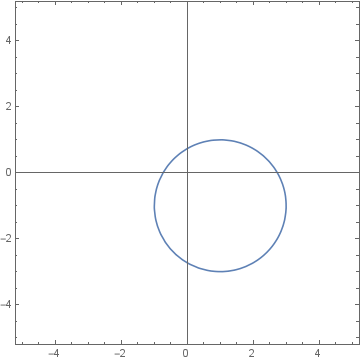
\includegraphics[scale=0.6]{123a.png}
			\end{figure}
			
		\skipitems{1}
		
		\item $\{z \in \mathbb{C} : \text{Re}(z + 2 - 2i)=3\}$
			\begin{figure}[H]
			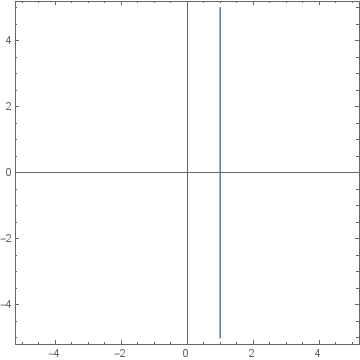
\includegraphics[scale=0.6]{123c.png}
			\end{figure}
			
		\item $\{z \in \mathbb{C} : |z-i|+|z+i|=3 \}$
			\begin{figure}[H]
			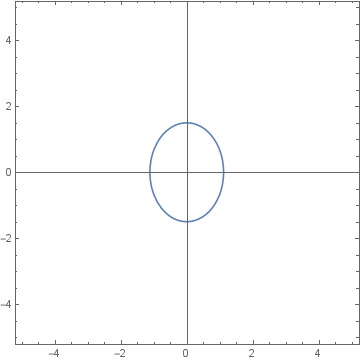
\includegraphics[scale=0.6]{123d.png}
			\end{figure}
			
		\skipitems{3}
		
		\item $\{z \in \mathbb{C} : \text{Im}(z^2)=1\}$
			\begin{figure}[H]
			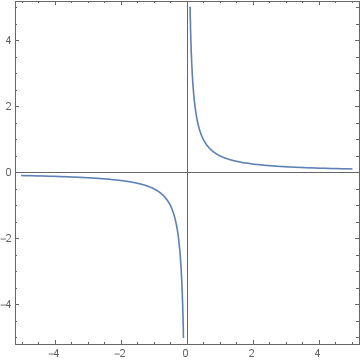
\includegraphics[scale=0.6]{123h.png}
			\end{figure}
	\end{enumerate}
	
	\item Sketch the following sets on the complex plane.
	
	\begin{enumerate}
		\item $0 \leq \text{arg z} \leq \frac{\pi}{4}$
			\begin{figure}[H]
			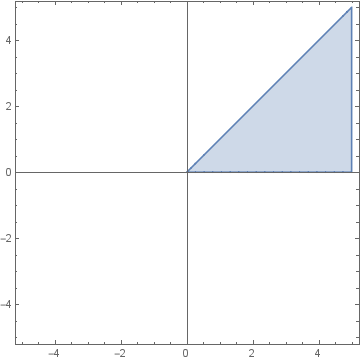
\includegraphics[scale=0.6]{6a.png}
			\end{figure}
		
		\item $\text{Re}(z^2) > 0$
			\begin{figure}[H]
			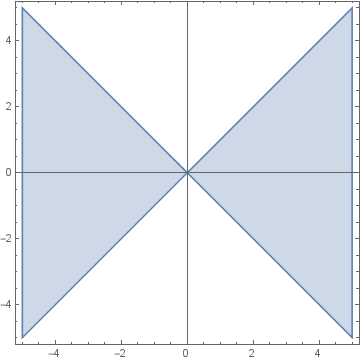
\includegraphics[scale=0.6]{6b.png}
			\end{figure}
			
		\item $0 < |z - 1| < 2$
			\begin{figure}[H]
			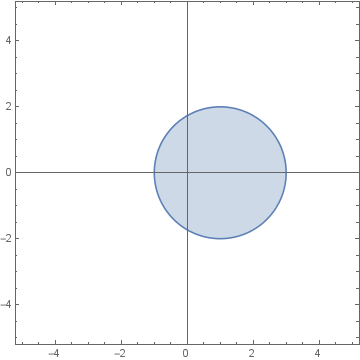
\includegraphics[scale=0.6]{6c.png}
			\end{figure}
		
		\item $|z| \leq |z-4|$
			\begin{figure}[H]
			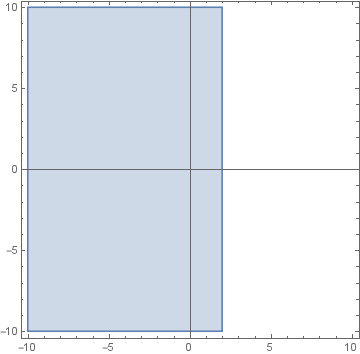
\includegraphics[scale=0.6]{6d.png}
			\end{figure}
	\end{enumerate}
	
	
	
\end{enumerate}
% ---------------------------------------------------
% Anything after the \end{document} will be ignored by the typesetting.
% ----------------------------------------------------

\end{document}

